
上一節的末尾,我們找出了程序在什麼地方花費了大部分的執行時間。在使用“明顯的”和“簡單的”優化後,出現了事與願違的情況,程序運行的更變慢了。現在很清楚,我們必須更詳細地研究性能的關鍵函數。

整個程序都在執行這段代碼,並且有方法來測試性能。至少在解決確定的性能問題之前是這樣,現在我們依舊對程序的其餘部分不再感興趣。

使用大型程序來優化幾行代碼有以下兩個缺點:

儘管這幾行代碼是性能關鍵的部分,但這並不意味著程序的其餘部分完全不需要時間(我們的示例中,確實需要。但是請記住,這個示例表示正在處理的整個大型程序)。可能要等上幾個小時,程序才能到達有趣的地方,要麼是因為整個任務都那麼長,要麼是因為性能關鍵函數只在特定條件下調用,比如:源於網絡的特定請求。

此外,處理大型程序需要更多的時間:編譯和鏈接時間更長。實際工作可能與其他開發者所做的代碼有交互,甚至編輯也需要更長時間,所以其他代碼會令人分心。因此,我們只對函數的基線感興趣,所以希望能夠調用這個函數,並進行測試。這就是\textbf{微基準測試}做的事情。

\subsubsubsection{2.5.1\hspace{0.2cm}微基準測試的基礎概念}

簡言之,微基準測試只是實現剛才描述目標的一種方式:運行一小塊代碼,並測試其性能。我們的例子中,其只是一個函數,但也可能是一個更雜的代碼段。重要的是,這段代碼可以在正確的初始條件下調用:對於函數,這些只是參數,但對於更大的代碼段,可能需要創建更復雜的內部狀態。

我們的例子中,確切地知道需要用什麼參數來調用字符串比較函數——我們構造了參數。需要做的第二件事是測試執行時間,我們已經瞭解了用於此目的的計時器。考慮到這一點,我們可以編寫一個非常簡單的基準測試,調用字符串比較函數的幾個變量,並報告結果:

\begin{lstlisting}[style=styleCXX]
bool compare1(const char* s1, const char* s2) {
	int i1 = 0, i2 = 0;
	char c1, c2;
	while (1) {
		c1 = s1[i1]; c2 = s2[i2];
		if (c1 != c2) return c1 > c2;
		++i1; ++i2;
	}
}
bool compare2(const char* s1, const char* s2) {
	unsigned int i1 = 0, i2 = 0;
	char c1, c2;
	while (1) {
		c1 = s1[i1]; c2 = s2[i2];
		if (c1 != c2) return c1 > c2;
		++i1; ++i2;
	}
}
int main() {
	constexpr unsigned int N = 1 << 20;
	unique_ptr<char[]> s(new char[2*N]);
	::memset(s.get(), 'a', 2*N*sizeof(char));
	s[2*N-1] = 0;
	system_clock::time_point t0 = system_clock::now();
	compare1(s.get(), s.get() + N);
	system_clock::time_point t1 = system_clock::now();
	compare2(s.get(), s.get() + N);
	system_clock::time_point t2 = system_clock::now();
	cout << duration_cast<microseconds>(t1 - t0).count() <<
	  "us " << duration_cast<microseconds>(t2 - t1).count() <<
	  "us" << endl;
}
\end{lstlisting}

這個程序中,只測試兩個比較函數,都沒有循環結束條件,一個用\texttt{int}型索引,另一個用\texttt{unsigned int}型索引。另外,我們不會在後面的代碼中重複\texttt{\#include}和\texttt{using}。輸入數據是一個長字符串,從頭到尾填充了相同的字符,所以子字符串的比較將一直進行到字符串的末尾。當然,可以根據需要的任何數據進行基準測試,我們先從最簡單的情況開始。

這個程序看起來是我們需要的事情:

%\hspace*{\fill} \\ %插入空行
\begin{center}
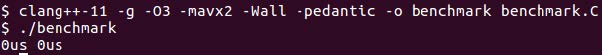
\includegraphics[width=0.9\textwidth]{content/1/chapter2/images/22.jpg}\\
圖 2.22
\end{center}

不管怎樣,都是0耗時。到底是哪裡出錯了呢?也許,單個函數調用的執行時間太快而無法測試?這是一個不錯的想法,我們可以很容易地解決這個問題:如果一個調用的時間太短,只需要多調用幾次:

\begin{lstlisting}[style=styleCXX]
int main() {
	constexpr unsigned int N = 1 << 20;
	constexpr int NI = 1 << 11;
	unique_ptr<char[]> s(new char[2*N]);
	::memset(s.get(), 'a', 2*N*sizeof(char));
	s[2*N-1] = 0;
	system_clock::time_point t0 = system_clock::now();
	for (int i = 0; i < NI; ++i) {
		compare1(s.get(), s.get() + N);
	}
	system_clock::time_point t1 = system_clock::now();
	for (int i = 0; i < NI; ++i) {
		compare2(s.get(), s.get() + N);
	}
	system_clock::time_point t2 = system_clock::now();
	cout << duration_cast<microseconds>(t1 - t0).count() <<
	  "us " << duration_cast<microseconds>(t2 - t1).count() <<
	  "us" << endl;
}
\end{lstlisting}

可以增加迭代次數\texttt{NI}直到得到結果,對吧?不可能那麼快的:

%\hspace*{\fill} \\ %插入空行
\begin{center}
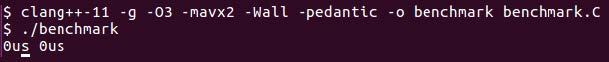
\includegraphics[width=0.9\textwidth]{content/1/chapter2/images/23.jpg}\\
圖 2.23
\end{center}

確實太快了,但為什麼呢?讓我們在調試器中逐步檢查這個程序,看看它實際上做了什麼:

%\hspace*{\fill} \\ %插入空行
\begin{center}
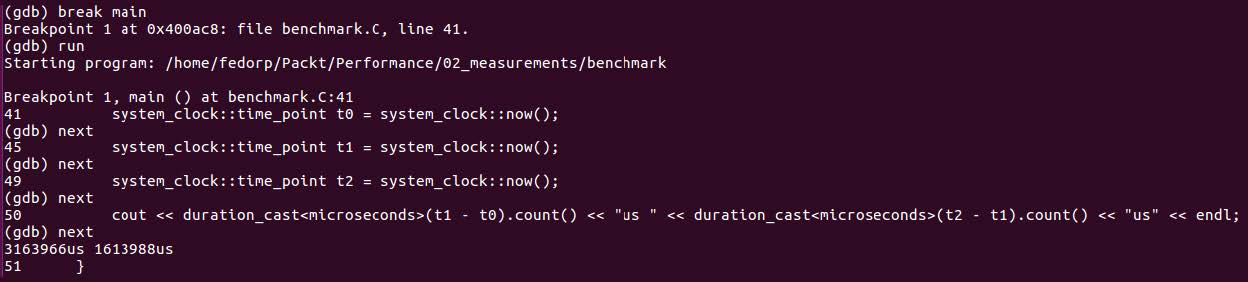
\includegraphics[width=0.9\textwidth]{content/1/chapter2/images/24.jpg}\\
圖 2.24
\end{center}

我們在\texttt{main}函數中設置了斷點,所以程序一啟動就會暫停,然後一行一行地執行程序……不過,這並不是我們寫的所有的代碼行!剩下的代碼在哪裡?我們可以猜測這是編譯器的原因,但是為什麼呢?我們需要了解更多關於編譯器優化的知識。

\subsubsubsection{2.5.2\hspace{0.2cm}微基準測試和編譯器優化}

要理解神祕的缺失代碼,我們必須看下這裡做了什麼。其創建一些字符串,調用比較函數,然後……沒有了?!沒有別的事情發生。除了在調試器中觀察代碼外,如何通過運行這個程序來知道代碼是否執行了呢?沒有其他辦法了。早在我們之前,編譯器得出了同樣的結論。因為編譯器已經對其進行了優化,所以開發者無法區分執行和不執行代碼的區別。但是,開發者可以分辨出的是,什麼都不做比做某事花費的時間要少得多。這裡,可以從C++標準中得到一個非常重要的概念,它對理解編譯器優化至關重要——可觀察行為。

標準表示,編譯器可以對程序進行更改,只要這些更改不會改變可觀察對象的行為即可。標準對於什麼構成了可觀察行為也非常具體:

\begin{enumerate}
\item 對易變(volatile)對象的訪問(讀和寫)需要嚴格按照發生它們的表達式的語義進行。特別是,對於同一線程上其他易變對象的訪問,編譯器不能重排。

\item 程序終止時,寫入文件的數據與寫入程序執行時的數據一樣。

\item 發送到交互設備的提示文本,將在程序等待輸入之前顯示出來。簡單地說,輸入和輸出操作不能省略或重排。
\end{enumerate}

上述規則有幾個例外,但沒有一個適用於我們的程序。編譯器必須遵循假設規則,經過優化的程序應該與所寫代碼的可觀察行為完全一樣,並一行一行地執行。請注意,因為調試器下運行程序並不構成可觀察行為,所以調試器中會有代碼缺失。它的執行時間很長,不執行看起來也無所謂,所以編譯器為了優化程序,就略過了執行。

在新的理解下,讓我們再來看看基準代碼。字符串比較的結果不會影響可觀察行為,因此整個計算可以由編譯器自行決定。我們的觀察也找到了解決這個問題的方法,必須確保計算的結果影響可觀察行為。一種方法是利用volatile語義:

\hspace*{\fill} \\ %插入空行
\noindent
\textbf{05\_compare\_timer.C}
\begin{lstlisting}[style=styleCXX]
int main() {
	constexpr unsigned int N = 1 << 20;
	constexpr int NI = 1 << 11;
	unique_ptr<char[]> s(new char[2*N]);
	::memset(s.get(), 'a', 2*N*sizeof(char));
	s[2*N-1] = 0;
	volatile bool sink;
	system_clock::time_point t0 = system_clock::now();
	for (int i = 0; i < NI; ++i) {
		sink = compare1(s.get(), s.get() + N);
	}
	system_clock::time_point t1 = system_clock::now();
	for (int i = 0; i < NI; ++i) {
		sink = compare2(s.get(), s.get() + N);
	}
	system_clock::time_point t2 = system_clock::now();
	cout << duration_cast<microseconds>(t1 - t0).count() <<
	  "us " << duration_cast<microseconds>(t2 - t1).count() <<
	  "us" << endl;
}
\end{lstlisting}

對比較函數的每次調用的結果都需要寫入volatile變量中,並且根據標準,這些值必須正確,且以正確的順序寫入。編譯器現在別無選擇,只能調用比較函數並獲得結果。只要結果本身不變,計算這些結果的方法仍然可以優化。這正是我們想要的,希望編譯器為比較函數生成最好的代碼,最好是在實際程序中生成的代碼,但不想讓它完全放棄這些功能。運行這個基準測試表明我們終於實現了目標,代碼肯定會運行:

%\hspace*{\fill} \\ %插入空行
\begin{center}
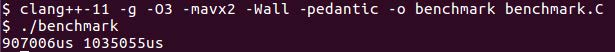
\includegraphics[width=0.9\textwidth]{content/1/chapter2/images/25.jpg}\\
圖 2.25
\end{center}

第一個值是\texttt{compare1()}函數的運行時,該函數使用\texttt{int}型索引,確實比\texttt{unsigned int}版本略快一些(暫時不要太相信這些結果)。

將我們的計算與某些可觀察行為綁定在一起的第二個選擇是,將結果打印出來,這可能會有點棘手。考慮一下簡單的修改:

\begin{lstlisting}[style=styleCXX]
int main() {
	constexpr unsigned int N = 1 << 20;
	constexpr int NI = 1 << 11;
	unique_ptr<char[]> s(new char[2*N]);
	::memset(s.get(), 'a', 2*N*sizeof(char));
	s[2*N-1] = 0;
	bool sink;
	system_clock::time_point t0 = system_clock::now();
	for (int i = 0; i < NI; ++i) {
		sink = compare1(s.get(), s.get() + N);
	}
	system_clock::time_point t1 = system_clock::now();
	for (int i = 0; i < NI; ++i) {
		sink = compare2(s.get(), s.get() + N);
	}
	system_clock::time_point t2 = system_clock::now();
	cout << duration_cast<microseconds>(t1 - t0).count() <<
	  "us " << duration_cast<microseconds>(t2 - t1).count() <<
	  "us" << sink << endl;
}
\end{lstlisting}

注意,變量\texttt{sink}不再是volatile類型。相反,我們輸出了最終值。不過,這並不像想象的那樣有效:

%\hspace*{\fill} \\ %插入空行
\begin{center}
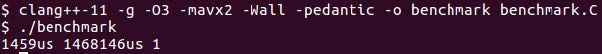
\includegraphics[width=0.9\textwidth]{content/1/chapter2/images/26.jpg}\\
圖 2.26
\end{center}

函數\texttt{compare2()}的執行時間與以前大致相同,但\texttt{compare1()}快太多了。目前為止,我們已經足夠瞭解這種虛假的“改進”。編譯器發現第二個調用覆蓋了第一個調用的結果,因此不會影響可觀察行為。

這就帶來了一個有趣的問題:為什麼編譯器沒有發現循環的第二次迭代與第一次的結果相同,並優化了第一次以外的所有對比較函數的調用,對於每個函數都會這樣麼?如果優化器足夠高級,那麼它可以做到,然後我們需要做更多的工作來繞過它。通常,將函數編譯為單獨的編譯單元就可以防止此類優化,儘管有些編譯器能夠進行整個程序的優化,所以在運行微基準測試時,可能要關閉這些特性。

注意,兩個基準測試運行產生了一些不同的值,甚至對於沒有優化的函數的執行時間也是如此。如果再次運行這個程序,可能會得到另一個值,也在相同的範圍內,但略有不同。這還不夠,我們需要的不僅僅是大概的數字。我們可以多次運行基準測試,計算需要重複多少次,並計算平均時間,但無需手工操作。不必編寫代碼來完成此任務,因為這樣的代碼已經有了,並且可以作為微基準測試工具使用。我們現在就來學習一種這樣的工具。

\subsubsubsection{2.5.3\hspace{0.2cm}谷歌基準測試工具}

編寫一個微型基準測試需要大量的樣板代碼,主要用於測試時間和結果累加。此外,該代碼對測試的準確性至關重要。現在,有幾個高質量的微基準庫可用。本書中,我們使用谷歌基準庫,下載和安裝該庫的說明可以在\textbf{相關準備}部分找到。本節中,我們將描述如何使用庫,並解釋結果。

使用谷歌基準庫,我們必須編寫一個小程序來準備輸入,並執行我們想要基準測試的代碼。這是一個基本的谷歌基準程序,用於測試字符串比較函數的性能:

\hspace*{\fill} \\ %插入空行
\noindent
\textbf{10\_compare\_mbm.C}
\begin{lstlisting}[style=styleCXX]
#include "benchmark/benchmark.h"
using std::unique_ptr;
bool compare_int(const char* s1, const char* s2) {
	char c1, c2;
	for (int i1 = 0, i2 = 0; ; ++i1, ++i2) {
		c1 = s1[i1]; c2 = s2[i2];
		if (c1 != c2) return c1 > c2;
	}
}
void BM_loop_int(benchmark::State& state) {
	const unsigned int N = state.range(0);
	unique_ptr<char[]> s(new char[2*N]);
	::memset(s.get(), 'a', 2*N*sizeof(char));
	s[2*N-1] = 0;
	const char* s1 = s.get(), *s2 = s1 + N;
	for (auto _ : state) {
		benchmark::DoNotOptimize(compare_int(s1, s2));
	}
	state.SetItemsProcessed(N*state.iterations());
}
BENCHMARK(BM_loop_int)->Arg(1<<20);
BENCHMARK_MAIN();
\end{lstlisting}

每個谷歌基準測試程序都必須包括庫的頭文件\texttt{benchmark/benchmark.h},還要包括編譯我們想要測量的代碼所需的其他頭文件(它們在前面的代碼清單中)。程序本身由許多基準測試“固件”組成,每一個都是一個具有特定簽名的函數,接受一個引用參數\texttt{benchmark::State},無返回值。該參數是谷歌基準庫提供的一個對象,可以讓外部開發者與基準庫進行對接。

對於每個代碼片段,需要一個固件,比如:想要進行基準測試的函數。在每個基準測試固件中,要做的第一件事是設置需要用作要運行的代碼輸入的數據。通常,需要重新創建這個代碼的初始狀態,以表示在實際程序中的狀態。我們的例子中,輸入是字符串,所以需要分配和初始化字符串。可以將字符串的大小硬編碼到基準測試中,但也有一種方法可以將參數傳遞到基準測試固件中。固件使用參數字符串長度,作為\texttt{state.range(0)}的值。當然,也可以傳遞其他類型的參數,詳細信息請參考谷歌基準庫的文檔。

基準測試上,整個設置是隨意的,因為不用測試準備數據所需的時間。測試執行時間的代碼在基準測試循環的主體中,\texttt{for (auto \_: state){…}}。較老的例子中,可以發現這個循環會寫成\texttt{while (state.KeepRunning()){…}},可以做著同樣的事情,但效率略低。基準庫來測試每次迭代所花費的時間,並決定要進行多少次迭代來累積足夠的數據,以減少在測試一小段代碼的運行時間時不可避免的隨機噪聲(只測試基準循環中代碼的運行時間)。

當測試足夠精確(或達到一定的時間限制)時,循環退出。對於循環,通常需要一些代碼來清理前面初始化的數據。我們的例子中,這個清理由\texttt{std::unique\_ptr}對象的析構函數進行。還可以調用\texttt{State}對象來輸出基準測試報告的結果,基準庫總是報告運行循環的一次迭代所花費的平均時間,但有時用其他方式表示程序的速度會更方便。字符串比較,一個選項是報告代碼每秒處理的字符數,可以通過調用\texttt{state}來實現。\texttt{SetItemsProcessed()}包含整個運行期間處理的字符數,每次迭代\texttt{N}個字符(若想要同時計算兩個子字符串,則為\texttt{2*N};項目可以計算已定義為處理單元的內容)。

不會因為定義了一個基準固件而發生任何事情,我們需要將它註冊到庫中。這裡使用\texttt{BENCHMARK}宏完成,宏的參數是函數名。這個名字沒有什麼特別,它可以是任何C++標識符;我們以\texttt{BM\_}開頭,只是遵循本書的命名慣例。\texttt{BENCHMARK}宏也是指定要傳遞給基準測試固件參數的地方,參數和其他基準的選項使用重載的箭頭操作符傳遞:

\begin{lstlisting}[style=styleCXX]
BENCHMARK(BM_loop_int)->Arg(1<<20);
\end{lstlisting}

這行代碼用參數\texttt{1<<20}註冊了基準固件\texttt{BM\_loop\_int},這個參數可以通過調用\texttt{state.range(0)}在固件中檢索。本書中,我們將看到更多不同參數的例子,可以在庫文檔中找到更多這樣的例子。

前面的代碼清單中沒有\texttt{main()}。不過,有另一個宏\texttt{BENCHMARK\_MAIN()},這裡\texttt{main()}不由我們來寫,而是由谷歌基準庫提供,它負責設置基準測試環境、註冊基準並執行基準。

回到我們的測量,並更仔細地觀察代碼:

\begin{lstlisting}[style=styleCXX]
for (auto _ : state) {
	benchmark::DoNotOptimize(compare_int(s1, s2));
}
\end{lstlisting}

\texttt{benchmark::DoNotOptimize(…)}包裝器的作用類似於之前使用的volatile型\texttt{sink}:可以確保編譯器不會優化掉對\texttt{compare\_int()}的調用。注意,它實際上並沒有關閉任何優化,括號內的代碼會進行優化,這是我們想要的。它確實是告訴編譯器表達式的結果,在我們的例子中,比較函數的返回值應該認為是“使用”,不能簡單地丟棄。

現在,我們已經準備好編譯,並運行第一個微基準測試了:

%\hspace*{\fill} \\ %插入空行
\begin{center}
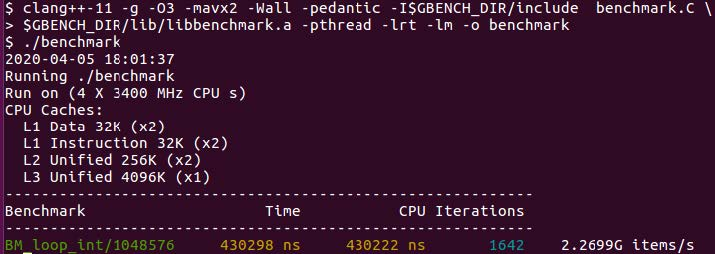
\includegraphics[width=0.9\textwidth]{content/1/chapter2/images/27.jpg}\\
圖 2.27
\end{center}

編譯時必須列出到谷歌基準的頭文件和庫路徑,而谷歌基準庫libbenchmark.a還依賴其他幾個庫。調用時,基準測試程序就會打印一些關於正在運行的系統的信息,然後執行每個已註冊的固件及其參數。每個基準固件會有一行輸出和一組參數,報告包括基準循環體的一次執行的平均實時時間和平均CPU時間、執行循環的次數,以及其他添加到報告中的統計信息(我們的例子中,是通過比較每秒處理的字符數,超過2G字符/秒)。每次運行這些數據會有變化嗎?如果使用正確的命令行參數啟用統計信息收集,那麼基準庫可以計算出這些數據,然後就可以進行比較了。

重複基準測試10次並報告結果,可以這樣:

%\hspace*{\fill} \\ %插入空行
\begin{center}
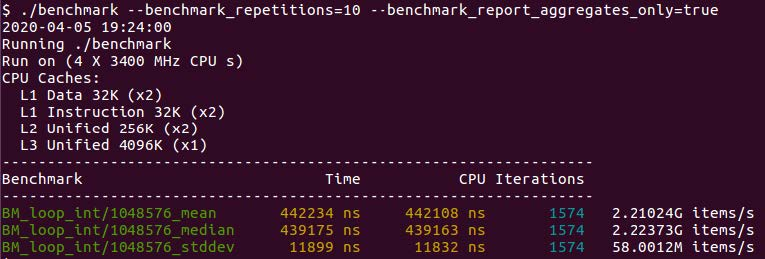
\includegraphics[width=0.9\textwidth]{content/1/chapter2/images/28.jpg}\\
圖 2.28
\end{center}

看來測量結果相當準確,標準差很小。我們可以比較函數的不同實現,並找出哪個是最快的。在這之前,得說個祕密。

\subsubsubsection{2.5.4\hspace{0.2cm}微基準測試不說實話}

做了多次微基準測試後,會很快會發現這麼說的原因。首先,結果是有意義的,因為做了很好的優化,一切看起來都很好。然後做一些小的改變,就會得到非常不同的結果。回去再進行檢查,現在測試給出了不同的數字。最後,會得到兩個幾乎相同的測試,但結果完全相反的結果,這會摧毀使用者對微觀基準的信任,而我唯一能做的就是摧毀它,但要以一種可控的方式,這樣我們還能從廢墟中搶撈出一些有用的東西。

微基準測試和其他性能指標的基本問題是,它們很大程度上依賴於上下文。隨著閱讀本書後續的部分,將瞭解現代計算機的性能行為是複雜的。結果不僅取決於代碼正在做什麼,還取決於系統其餘部分在做什麼,取決於它之前在做什麼,以及在代碼到達興趣點之前執行的路徑。這些東西在微觀基準測試中,都不會進行復刻。

相反,基準有自己的上下文。基準測試庫的作者並不是沒有意識到這個問題,他們儘可能地去解決這個問題。谷歌基準庫在每個測試上都進行了長期測試:最初的幾個迭代可能具有與運行的其餘部分非常不同的性能特徵,因此庫會忽略最初的測量值,直到結果“穩定下來”。但這也定義了一個特定的上下文,可能與實際的程序不同。實際的程序中,對函數的每次調用只重複一次(另一方面,有時會在整個程序運行過程中多次使用相同的參數調用同一個函數,所以這可能會有不同的上下文)。

運行基準測試之前,無法在每個細節上忠實地再現大型程序的真實環境,但是有些細節很重要。上下文差異的最大來源是編譯器,或是編譯器對實際程序和微基準的優化。我們知道編譯器試圖指出,微基準測試上運行非常慢的方法,沒有做任何有用的事情(或至少沒有可觀察的),然後會用更快的方法來替換它。之前使用的\textit{DoNotOptimize}包裝器解決了一些由編譯器優化引起的問題。

編譯器仍有可能發現對函數的每次調用都返回相同的結果。此外,由於函數定義與調用在同一個文件中,編譯器可以內聯整個函數,並使用收集到的信息來優化函數。通常情況下,當從另一個編譯單元調用函數時,這種優化不可用。

為了在微基準測試中更準確地還原真實情況,可以將比較函數移動到它自己的文件中,並編譯它。我們有一個文件(編譯單元),只有基準測試固件:

\hspace*{\fill} \\ %插入空行
\noindent
\textbf{11\_compare\_mbm.C}
\begin{lstlisting}[style=styleCXX]
#include "benchmark/benchmark.h"
extern bool compare_int(const char* s1, const char* s2);
extern bool compare_uint(const char* s1, const char* s2);
extern bool compare_uint_l(const char* s1, const char* s2,
unsigned int l);
void BM_loop_int(benchmark::State& state) {
	const unsigned int N = state.range(0);
	unique_ptr<char[]> s(new char[2*N]);
	::memset(s.get(), 'a', 2*N*sizeof(char));
	s[2*N-1] = 0;
	const char* s1 = s.get(), *s2 = s1 + N;
	for (auto _ : state) {
		benchmark::DoNotOptimize(compare_int(s1, s2));
	}
	state.SetItemsProcessed(N*state.iterations());
}
void BM_loop_uint(benchmark::State& state) {
	… compare_uint(s1, s2) …
}
void BM_loop_uint_l(benchmark::State& state) {
	… compare_uint_l(s1, s2, 2*N) …
}
BENCHMARK(BM_loop_int)->Arg(1<<20);
BENCHMARK(BM_loop_uint)->Arg(1<<20);
BENCHMARK(BM_loop_uint_l)->Arg(1<<20);
\end{lstlisting}

可以單獨編譯文件,並將它們鏈接在一起(必須關閉所有的程序優化)。現在,我們有了一個合理的預期,因為無法計算出基準測試中使用的參數,編譯器不會生成子字符串比較的簡化版本。通過這個簡單的措施,結果就與我們在分析整個項目時所觀察到的情況更加一致:

%\hspace*{\fill} \\ %插入空行
\begin{center}
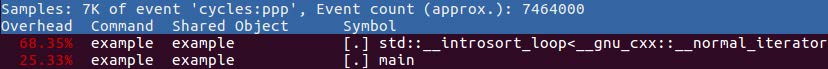
\includegraphics[width=0.9\textwidth]{content/1/chapter2/images/29.jpg}\\
圖 2.29
\end{center}

代碼的初始版本使用了\texttt{unsigned int}索引作為循環中的邊界條件(最後一行),只要邊界條件檢查有不必要的檢查就會導致性能下降(中間一行)。最後,將索引更改為\texttt{signed int}就可以恢復丟失的性能,甚至可以提高性能(第一行)。

單獨編譯代碼段通常足以避免不必要的優化。通常,會發現編譯器會根據同一文件中的其他內容對特定的代碼塊進行優化。這可能只是編譯器中的Bug,但也可能是一些啟發式的結果,根據編譯器編寫者的經驗,這通常是正確的。觀察到結果取決於一些沒有執行的代碼,因為是編譯,這只是可能的原因。解決方案會使用實際程序中的編譯單元,調用需要進行基準測試的函數就可以了。當然,必須滿足編譯和鏈接依賴項,因此這裡還需要編寫模塊化代碼,並最小化依賴項。

其他上下文是計算機本身的狀態。如果整個程序耗盡了內存,並在交換中循環,那麼小內存的基準測試將不能代表真正的問題;另一方面,現在的問題不在“慢”代碼中,問題是在其他方面消耗了太多的內存。這種上下文依賴還有更微妙的版本,並且可能會影響基準測試。這種情況是,結果取決於執行測試的順序(微基準測試中,則為\texttt{BENCHMARK}宏的順序)。重新排序測試或只運行測試的子集可能會得到不同的結果,它們之間存在某種依賴關係。可以是代碼依賴項,通常與某些全局數據結構中的數據積累一樣簡單,這可能是對硬件狀態的依賴。這些情況很難理解,在本書的後面,將瞭解一些導致這種依賴的原因。

最後,有一個上下文依賴的主要來源掌握在測試者手中(這未必容易避免,但至少是可以避免的),它依賴於程序的狀態。我們需要處理這種依賴,要對輸入進行基準測試。有時,輸入是已知的或可以重構的。通常,性能問題只會發生在特定類型的輸入上,我們不知道它們有什麼特別之處,直到分析了在這些特定輸入情況下的代碼性能(這正是我們用微基準測試所要做的事情)。這種情況下,通常最容易從實際程序的運行中獲取輸入,並將它們存儲在文件中,使用它們重新創建測試代碼的狀態。這個輸入可以是簡單的數據集合,也可以是複雜的事件序列,這些事件序列需要記錄並“回放”到事件處理程序中,以重現相應的行為。

我們需要重構的狀態越複雜,在微基準測試中再現真實程序的性能行為就越困難。這個問題有點類似於編寫單元測試,若程序不能以更簡單的狀態分解成更小的單元,那麼編寫單元測試也要困難得多。這裡,我們看到了設計良好的軟件系統的優點,具有良好單元測試覆蓋率的代碼庫通常更容易進行微基準測試。

正如在本節開始時所警告的那樣,它的目的是在一定程度上是要恢復對微基準測試的信心。微基準測試是一個有用的工具,但它們也會把你引入歧途,有時甚至會走得很遠。現在,請理解其中的原因,並更好地準備從結果中獲取有用的信息,而不是完全放棄微基準測試。

我們在本章中介紹的工具沒有一個能解決所有問題,它們不是萬金油。而我們可以通過使用這些工具,以各種方式收集信息來達到最佳的效果,因此它們之間是相輔相成的。






